\documentclass[11pt,letterpaper]{article}
%%%%%\usepackage{cite}
\usepackage{amsmath}
\usepackage{amsfonts}
\usepackage{array}
\usepackage{dsfont}
\usepackage{amssymb}
\usepackage{amsthm}
\usepackage{bbold}
\usepackage{fullpage}
\usepackage{mathtools}
\usepackage{enumitem}
\usepackage{mathrsfs}
\usepackage[margin=0.9 in,headsep=0.3 in]{geometry}
\usepackage{hyperref}
\usepackage{graphicx}
\usepackage{gensymb}
\usepackage{xcolor,colortbl}
\usepackage[format=plain,
labelfont={bf,it},
textfont={it}]{caption}
\usepackage{float}
\usepackage{multirow}

\usepackage[backend=biber, style=ieee]{biblatex}
\addbibresource{Bibliography.bib}

%%%%%%%%%%%NEW PACKAGES I'VE ADDED FOR THE PURPOSE OF THESIS
\usepackage{amsthm}
\theoremstyle{definition}
\newtheorem{defn}{Definition}[section] % definition numbers are dependent on theorem numbers

\usepackage{newclude}
\usepackage{tikz}
\usetikzlibrary{shapes.geometric, arrows}
%%Define the two block types and arrow type for our flow diagram
\tikzstyle{startstop} = [rectangle, rounded corners, minimum width=3cm, minimum height=1cm,text centered, draw=black, fill=white]
\tikzstyle{process} = [rectangle, minimum width=3cm, minimum height=1cm, text centered, draw=black, fill=white]
\tikzstyle{arrow} = [thick,->,>=stealth]
%%%%%%%%%%%END OF NEW PACKAGES I'VE ADDED FOR THE PURPOSE OF THESIS

\newcommand*{\SignatureAndDate}[1]{%
	\par\noindent\makebox[2.5in]{\hrulefill} \hfill\makebox[2.0in]{\hrulefill}%
	\par\noindent\makebox[2.5in][l]{#1}      \hfill\makebox[2.0in][l]{Date}%
}%
\newcolumntype{L}{>{\centering\arraybackslash}m{2cm}}
\newcolumntype{P}{>{\centering\arraybackslash}m{3cm}}
\newcolumntype{Q}{>{\centering\arraybackslash}m{4cm}}
\setlength{\parindent}{0em}

\allowdisplaybreaks

\newcommand{\R}{\mathds{R}}
\newcommand{\Z}{\mathds{Z}}
\newcommand{\Rplus}{\mathds{R}_{> 0}}
\newcommand{\Zplus}{\mathds{Z}_{\geq 0}}
\newcommand{\F}{\mathds{F}}
\newcommand{\N}{\mathds{N}}
\newcommand{\T}{\mathds{T}}
\newcommand{\s}{\mathds{S}}
\newcommand{\C}{\mathds{C}}
\newcommand{\CDFT}{\mathscr{F}_{CD}} %Fourier transform
\newcommand{\ip}[2]{\langle #1, #2\rangle}

\setlength{\parskip}{0.5em}

\usepackage{fancyhdr}
\setlength{\headheight}{15.2pt}
\pagestyle{fancy}
%%\fancyhead[RE]{\thepage}
%%\fancyhead[ER]{\rightmark}
\fancyhead[LE,RO]{\slshape \rightmark}
\fancyhead[LO,RE]{\slshape \leftmark}
\fancyfoot[C]{\thepage}

\makeatletter
\newsavebox\myboxA
\newsavebox\myboxB
\newlength\mylenA

\title{ A-1: Modelling and Control of a Ripstik\textsuperscript{\textregistered} \\MTHE 493 Final Report}
\date{Friday April $7^{\textrm{th}}$, 2017}
\author{\\Andrew Cantanna (10092489) \\Cameron Hudson (10092287)\\
	Benjamin Rudson (10083664)\\}
\begin{document}

	\begin{titlepage}
		\maketitle
		\thispagestyle{empty}		
	\end{titlepage}
	\newpage
	\pagenumbering{Roman} 
	%%\pagestyle{myheadings}
\begin{abstract}
	This is the abstract.
\end{abstract}	
\clearpage
\newpage
\centering
\paragraph{Acknowledgements}

\newpage	
	\renewcommand{\baselinestretch}{0.75}\normalsize
	\tableofcontents
	\renewcommand{\baselinestretch}{1.0}\normalsize

\newpage
\listoffigures
\newpage
\listoftables


\clearpage
\pagenumbering{arabic}
	
	\newpage



	\pagestyle{fancy}
\section{Introduction}
\subsection{Context \& Motivation}
%Introduce most of the concepts around money in electric transportation/urbanization/environmental aspects from the presentation, e.g. "why is this needed"
\subsubsection{The RipStik}
\subsection{Problem Definition}
\subsection{Technical Background}
\subsubsection{Euler Angles}
\subsubsection{Lagrangian Mechanics}
\subsubsection{Euler-Lagrange Equations}
\subsubsection{Nonholonomic Constraints}
\subsubsection{Numeric Integration}
\subsubsection{Linear Quadratic Regulator Control}
The linear quadratic regulator (LQR) algorithm is a method in control theory used to technique used to determine the optimal control gains for a state feedback controller for a linear system with a quadratic cost function. \textbf{CITE LAB MANUAL OR SOMETHING}

For the purpose of this project, linear control systems $\Sigma$ of the form
\begin{equation}
\dot{x}(t) = Ax(t) + Bu(t)
\end{equation}
where $A \in \R^{m \times m}$ and $B \in \R^{m \times l}$ are considered.
The associated quadratic cost function is then 
\begin{equation}
\eta(u) = \int_{0}^{\infty}x^{T}(t)Qx(t)+u^{T}(t)u(t)dt
\end{equation}
where $Q \in \R^{m \times m}$ is the weighting matrix associated with the degrees of freedom and their derivatives $(q, \dot{q})$ in the system. Note that no weightings are associated with the control inputs at this stage, though they may be necessary when considering the broader design impacts (see section \textbf{FILL IN SECTION REF}). Tuning the cost function weighting matrix $Q$ allows emphasis to be placed on stabilization of certain degrees of freedom to better meet design goals for the particular application.

The optimal control gains $K$ are then computed from
\begin{equation}
K = B^{T}X_{r}
\end{equation}
where  $X_{r}$ is the solution to the continuous Riccati equation \textbf{CITE MATHEMATICA DOCS FOR RICCATISOLVE}
\begin{equation}
A^{T}X_{r} + X_{r}A - (X_{r}B)(B^{T}X_{r}) + Q = 0.
\end{equation}

\subsection{Literature Review}
\subsubsection{A Nonlinear Mathematical Model for a Bicycle}
To gain a clearer perspective of the overall procedure and concepts involved in modeling a complex mechanical system of this nature, a number of similar mathematical models for other modes of personal transportation were analyzed.
In particular, \textit{A Nonlinear Mathematical Model for a Bicycle} \cite{bicycle} provides a clear example of establishing the necessary coordinate systems and transformation matrices associated with the interconnections and internal angles within the bicycle.
This model includes the rolling dynamics of the wheels and discusses the minutiae of elements like the wheel crown radius, demonstrating the complexity they add to the model before removing these elements to provide a more manageable model.
The final model is also constructed under the assumption that the rider remains stable and upright, allowing the roll angle of the bicycle to be linearized, further facilitating interpretation of the final modeling results. 
%%%%%%%%%%%%%%%%%%%%%%%%%%%%%%%%
%%%%SHOULD WE INCLUDE AN IMAGE
%%%%Is wheel crown radius not self explanatory
%%%%%%%%%%%%%%%%%%%%%%%%%%%%%%%%

\subsubsection{Modeling and Control of Casterboard Robot}
In the paper \textit{Modeling and Control of Casterboard Robot} \cite{robot}, Kinugasa et al. discuss similar concepts and their application in the context of a casterboard, however, the overarching goals and product were distinct from the defined problem.
The group from Osaka University developed a highly simplified model, omitting the problem of stability and simplifying the dynamics of the caster rotation using a holonomic constraint. 
They then used this to develop a locomotion control method for the casterboard before implementing, testing and tuning it on a physical robot constructed to match the geometry of the casterboard.

%%%%%%%%%%%%%%%%%%%%%%%%%%%%%%%%
%%%%SHOULD WE INCLUDE AN IMAGE
%%%%%%%%%%%%%%%%%%%%%%%%%%%%%%%%
\subsubsection{Nonholonomic Constraints \& Linearization}
%%%%%%%%%%%%%%%%%%%%%%%%%%
%%%%
%%%%FUCK IT I'LL DO THIS LATER IDK
%%%%
%%%%%%%%%%%%%%%%%%%%%%%%%%
\subsection{Software Tools}
\subsubsection{Mathematica}
Due to the complex nature of the model and the large number of degrees of freedom needed to accurately model the behavior of the RipStik, a powerful symbolic computation tool is required to derive and manipulate the expressions. 
Mathematica was ultimately selected over other options such as Maple and the Matlab Symbolic toolbox due to the combination of robust symbolic and numeric computation features with easy to use visualization features for graphically displaying the various systems developed over the course of the project.
It also provided equivalent or better performance with thorough documentation and examples compared to competitors.
%%%%%%%%%%%%%%%%%%%%%%%%
%%%%DO I NEED A SOURCE FOR BETTER PERFORMANCE
%%%%%%%%%%%%%%%%%%%%%%%%
\subsubsection{Three.JS}
While all of the more simple visualizations were constructed directly in Mathematica, an external tool was constructed to animate the full RipStik system in a more attractive and visually intuitive manner. 
The application is javascript based and operated via the web browser, allowing the user to upload a .csv (comma separated value) file of numeric output from the RipStik simulation and returning an animation of the results on a 3 dimensional RipStik model. 
This allows easy validation of the results by inspection, particularly for complex motions where graphs of the angles and positions may not make the full system behavior immediately obvious.
The process used to generate these animations in the application is shown in Figure \ref{fig:ThreeJsFlow}.

%%Define the two block types and arrow type for our flow diagram
\tikzstyle{startstop} = [rectangle, rounded corners, minimum width=3cm, minimum height=1cm,text centered, draw=black, fill=white]
\tikzstyle{process} = [rectangle, minimum width=3cm, minimum height=1cm, text centered, draw=black, fill=white]
\tikzstyle{arrow} = [thick,->,>=stealth]
\begin{center}
	\begin{figure}[!htb]
		\begin{center}
			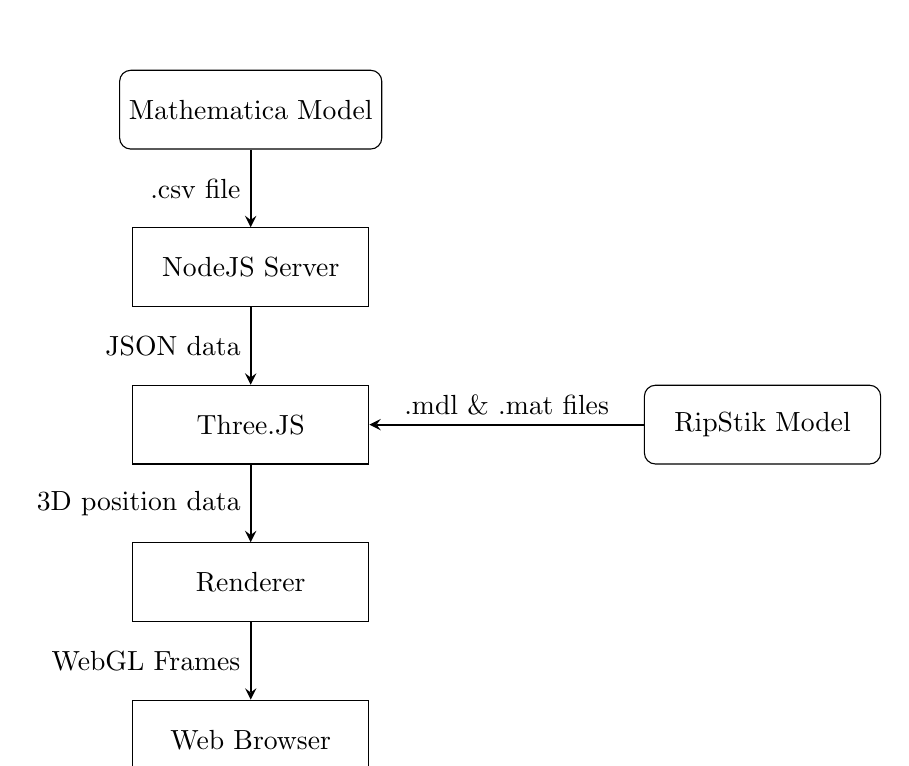
\begin{tikzpicture}[node distance=2cm]
				\node (WA) [startstop] {Mathematica Model};
				\node (Srvr) [process, below of=WA] {NodeJS Server};
				\node (Three) [process, below of=Srvr] {Three.JS};
				\node (Mdl) [startstop, right of=Three, xshift=4.5cm] {RipStik Model};
				\node (Rndr) [process, below of=Three] {Renderer};
				\node (Brwsr) [process, below of=Rndr] {Web Browser};

				\draw [arrow] (WA) -- node[anchor=east] {.csv file} (Srvr);
				\draw [arrow] (Srvr) -- node[anchor=east] {JSON data} (Three);
				\draw [arrow] (Mdl) -- node[anchor=south] {.mdl \& .mat files} (Three);
				\draw [arrow] (Three) -- node[anchor=east] {3D position data} (Rndr);
				\draw [arrow] (Rndr) -- node[anchor=east] {WebGL Frames} (Brwsr);
			\end{tikzpicture}
		\end{center}
	\caption{RipStik animation tool data flow summary}\label{fig:ThreeJsFlow}
	\end{figure}
\end{center}
The core of the application is ThreeJS, a javascript WebGL library that allows the 3D model to be loaded from a .mdl file (the set of 3D dimensional points that forms the shape) and .mat file (the colors/materials to be overlaid on the shape) then animated using rotations and translations in a standard Cartesian coordinate system.
\section{Design Methodology}
Throughout the project, an emphasis was placed on an iterative, test-driven design process. This testing involved both the use of smaller, well understood test cases and incremental unit tests in the context of the full system. 
The applicability of these smaller test cases stemmed from the use of the \textit{modular programming} paradigm, which allowed the same code to be used across a variety of different mechanical systems. 
The core principals and importance of these concepts will be briefly outlined before formalizing the overarching process.
\subsection{Modular Program Design}
The core principle of modular program design is to decompose the larger system design problem into small, independent modules\cite{Modular}.
An effective decomposition is done in such that the modules are have well defined inputs and outputs and can be tested independently, improving the flexibility of the application\cite{Modular}.
In designing the RipStik model, these modules are user created Mathematica functions, separated to each contain a complete, testable portion of the larger model.

Two alternate approaches were also considered but deemed unsuitable. Object Oriented design involves grouping related functionality and data, like parameters or variables, into larger "objects"\cite{ObjectOriented}.
This would provide similar compartmentalization \cite{ObjectOriented} but does not conform to the broader functional design of Mathematica \cite{MathematicaFunctional} and is less intuitive and legible for new users attempting to adopt code from the system. 

Alternately, a purely procedural approach would simply focus on laying out the set of commands sequentially in a single structure. 
This design would be more intuitive to new users and would likely improve initial development speed due to the lack of unit testing and reduced need for flexibility of the commands in sequence versus those implemented in independent modules.
Despite these benefits, this design was not selected since it would reduce the flexibility and testability of the system due to the purpose built nature of commands. 
This would make smaller test cases much more difficult to implement since each would be a completely independent code base with no shared functions outside of those central to Mathematica.
\subsection{Test Cases}
In order to validate each module during development, small test systems were developed. Each test system had to:
\begin{itemize}
\item Succinctly demonstrate the complete functionality of the module 
\item Be small and straightforward to minimize the time expended on setting up systems outside of the core RipStik model
\item Provide results that could be easily verified through simple visualizations and (where possible) published results
\end{itemize}
These test cases will be presented throughout the development of the model alongside the discussion of implementing each mathematical tool.
\subsection{Unit Testing}
In addition to the simple mechanical systems used to test each model, a test or set of tests was developed for the RipStik system to further validate that the given portion of the model was functioning as expected. These were designed to be as simple and easy to implement as possible while still testing the module as thoroughly as possible.
\subsection{Overall Process}
Together, these elements make up the core design process for each module as outlined in Figure \ref{fig:ProcessFlow}. These modules were then used to iteratively construct the overall RipStik model, adding functionality and testing incrementally for each mathematical tool applied.
\begin{center}
	\begin{figure}[!htb]
		\begin{center}
			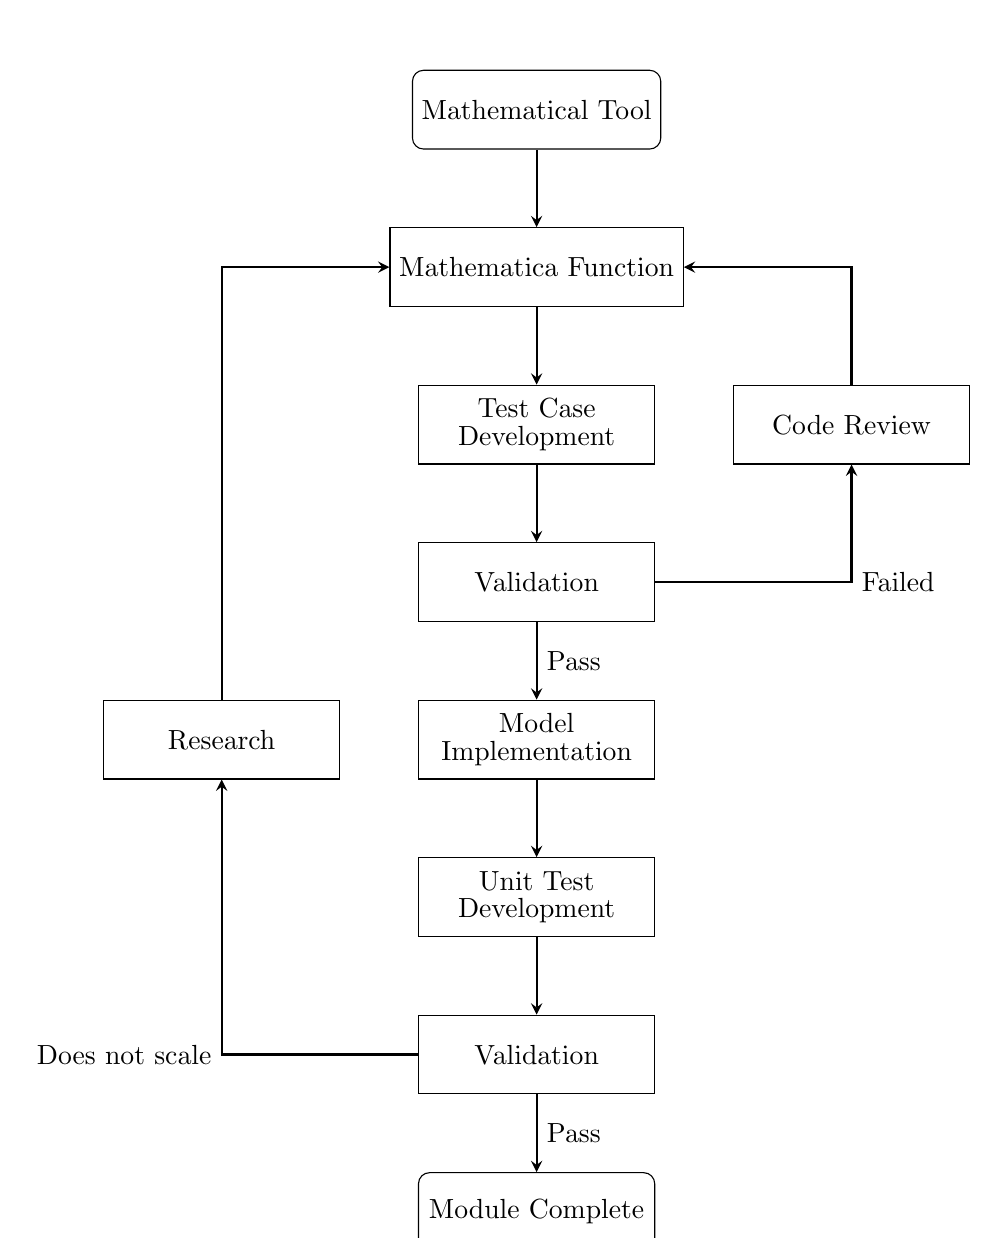
\begin{tikzpicture}[node distance=2cm]
				\node (math) [startstop] {Mathematical Tool};
				\node (code) [process, below of=math] {Mathematica Function};
				\node (testcase) [process, below of=code] {\shortstack{Test Case \\ Development}};
				\node (tcvalid) [process, below of=testcase] {Validation};
				\node (model) [process, below of=tcvalid] {\shortstack{Model \\ Implementation}};
				\node (unittest) [process, below of=model] {\shortstack{Unit Test \\ Development}};
				\node (utvalid) [process, below of=unittest] {Validation};
				\node (done) [startstop, below of=utvalid] {Module Complete};
				\node (research) [process, left of=model, node distance=4cm] {Research};
				\node (review) [process, right of=testcase, node distance=4cm] {Code Review};
				\draw [arrow] (math) -- (code);
				\draw [arrow] (code) -- (testcase);
				\draw [arrow] (testcase) -- (tcvalid);
				\draw [arrow] (tcvalid) -- node [anchor=west] {Pass}(model);
				\draw [arrow] (model) -- (unittest);
				\draw [arrow] (unittest) -- (utvalid);
				\draw [arrow] (utvalid) -- node [anchor=west] {Pass}(done);
				\draw [arrow] (utvalid) -| node [anchor=east] {Does not scale}(research);
				\draw [arrow] (research) |- (code);
				\draw [arrow] (tcvalid) -| node [anchor=west] {Failed}(review);
				\draw [arrow] (review) |- (code);
			\end{tikzpicture}
		\end{center}
	\caption{Design Process Summary Diagram}\label{fig:ProcessFlow}
	\end{figure}
\end{center}

\section{Development}
\subsection{Design Methodology}
%Introduce most of the concepts around money in electric transportation/urbanization/environmental aspects from the presentation, e.g. "why is this needed"
\subsection{Model Development}
\subsubsection{Core Assumptions}
\subsubsection{Coordinate Systems}
\paragraph{Test Case}
\paragraph{Model Implementation}
\paragraph{Validation}
\subsubsection{Equations of Motion}
\paragraph{Test Case}
\paragraph{Model Implementation}
\paragraph{Validation}
\subsubsection{Nonholonomic Constraints}
\paragraph{Test Case}
\paragraph{Model Implementation}
\subsubsection{Numeric Integration}
\paragraph{Evaluation}
\paragraph{Validation}
\subsubsection{Linear Quadratic Regulator Control}
\paragraph{Test Case}
\paragraph{Model Implementation Challenges}
\paragraph{Proposed Testing Framework}
\section{Engineering Considerations}
\subsection{Legal Considerations}

\subsubsection{Regulatory Considerations}

\paragraph{Street Legality}\mbox{}\\
Many jurisdictions have laws and regulations pertaining to the operation of personal transport vehicles, both electric and human-powered. 
Toronto and Fredricton are among many Canadian cities which have laws prohibiting the use of skateboards on public streets. \textbf{CITE? 3Chantale Nicole}
With regards to motorized transport, California had a long-standing ban on motorized skateboards which was recently abolished in the passing of Assembly Bill 2054 in 2015. \cite{OCLaws} \cite{WSJLaws}
Recently, the emergence of two-wheeled, self balancing electric scooters prompted the development of new laws and regulations. 
These devices are banned from airlines in Canada and the USA and their usage is heavily restricted or banned in regions including Toronto, Vancouver, New York City, and the state of California. \cite{leetboard}
It is imperative that a personal electric transport vehicle be compliant with relevant regulations and laws in its area of operation.


\paragraph{Intellectual Property}\mbox{}\\
In order to ensure that a personal electric transport system is commercially feasible, it is imperative that all the appropriate measures to protect intellectual property be undertaken. 
As the final product will involve the incorporation of mechanical control system to a pre-existing complex mechanical vehicle, the final product will qualify as a combinatory invention. 
A combinatory invention involves combining two or more pre-existing technologies in order to develop a new technology. 
Combinatory inventions are among the most common patents; between the years 1790 and 2010, 77\% of all patents granted involved the combination of at least two pre-existing technologies. \cite{COMB} 
A patent shall not be issued, under United States patent law, if \emph{the subject matter as a whole would have been obvious at the time the invention was made to a person having ordinary skill in the art to which said subject matter pertains. 
	Patentability shall not be negatived by the manner in which the invention was made.}" \cite{NonObv} 
\\
\\
A 2007 United States Supreme Court ruling in "KSR International Co. v. Teleflex Inc." established legal precedent for "non-obviousness" in combinatory inventions. 
Teleflex Inc. sued KSR International Co. for patent infringement pertaining to a KSR product which Teleflex claimed infringed on its patent for an "Adjustable Pedal Assembly with Electronic Throttle Control."
KSR argued that Teleflex's claim was invalid as the action was obvious. 
The United States Supreme Court ruled in favour of KSR International Co.,  
ruling that Teleflex's invention was not patentable as the combination of the two adjustable pedal assembly and the electronic throttle control was indeed obvious. 
\\
\\
In developing novel methods of personal electric transport, it is imperative that the designers consider existing patent laws and cases in order to ensure that their products can be protected.

\subsubsection{Professional Practice Considerations}
\subsection{Design Considerations}
%%Safety vs Power, cost vs power, battery life vs environmental considerations & power & cost, stability vs mobility, cost vs sustainability
\subsection{Ethics}
%Manufacturing, disposal, safety???, Marketing???
\subsection{Economic Analysis}
\subsubsection{Cost Breakdown}
In order to determine the economic feasibility of an electric transport device, it was compared to traditional gas and human powered transportation devices.
An analysis was conducted based on three different metrics; Initial cost, maintenance cost and fuel cost.
The electric powered devices used in the analysis were the OneWheel and Boosted board.
The Gas powered device used in the analysis was a 2017 Yamaha Zuma 50F.
The human powered device used in the analysis was a  Raleigh Furley bicycle.
\par
Initial cost looked at the upfront costs associated with purchasing each of the devices.
Maintenance cost looked at the necessary costs required for spare parts, and yearly upkeep of each device. 
Fuel costs looked at the cost required to power each of the devices.	
The economic analysis for each method was conducted over a span of five years, and the results can be seen in Table \ref{table:econ}.

\begin{table}[ht]
	\caption{Comparison of electric, gas, and human powered transportation devices over five years (all values in USD)}
	\centering
	\def\arraystretch{1.5}
	\begin{tabular}{|c| c| c| c| c|}
		\hline\hline
		\textbf{Method} & \textbf{Device}	& \textbf{Initial Cost (\$)} & \begin{tabular}{@{}c@{}} \textbf{Maintenance}\\ \textbf{Cost (\$)} \end{tabular} & \begin{tabular}{@{}c@{}} \textbf{Fuel} \\ \textbf{Cost (\$)} \end{tabular} \\ 
		\hline
		\multirow{2}{*}{Electric Powered} & OneWheel & 1,299 - 1,499 & 340 & 25 \\
		\cline{2-5}
		& Boosted Board & 1,299 - 1,499 & 359 & 25\\
		\hline
		Gas Powered & Yamaha Zuma 50F & 2,599 & 371.40 & 155\\ 
		\hline
		Human Powered & Raleigh Furley Bicycle & 980 & 969.90 & 0\\[0.1ex]	
		\hline
	\end{tabular}
	\label{table:econ}
\end{table}

The inital cost for the OneWheel was US\$1299.00 for the base model, and US\$1499.00 for the Plus model \cite{wheelcost}.	
The initial cost for the Boosted Board was US\$1299.00 for the base model, and US\$1499.00 for the plus model \cite{boardcost}.
The initial cost for the Yamaha Zuma 50F was US\$2,599.00 for the base model \cite{Yamaha}.
The initial cost for the Raleigh Furley Bicycle was US\$980.00 \cite{Raleigh}. 
The Raleigh was selected since it was ranked one of the top commuter bicycles for 2016 \cite{BikeMagazine}.
\par
The maintenance cost for the OneWheel totaled to US\$340.00, and consisted of one replacement charger (US\$125.00), and one tune up and reload pack (US\$215.00) \cite{wheelcost}.
The tune up and reload pack consisted of a 17 point inspection, motor, battery health, hardware and firmware assessment, new footpads, new bumpers, and a new tire \cite{wheelcost}.
The maintenance cost for the boosted board totaled to US\$359.00, and consisted of replacement parts for each of the key components on the board. This includes US\$105.00 for a full set of replacement wheels, US\$100.00 for a replacement remote, US\$79.00 for a replacement charger, US\$50.00 for a bearing service kit, and US\$25.00 for a motor belt service kit \cite{boardcost}.
The maintenance cost for the Yamaha Zuma 50F consisted of a maintenance kit with lube, oil filters, fuel filters,drain plugs, and a disposable funnel \cite{YamahaMaintenance}. 
This led to a cost of US\$74.28 per year, totaling to US\$371.40.
The maintenance cost for the Raleigh Furley bicycle consisted of a tune up and drivetrain clean, along with two new tires each year. 
The tune up and drivetrain clean cost US\$150.00 per year, totaling to US\$750.00 dollars \cite{bikerepair}. 
The replacement tires cost US\$44.00 per year, and totaled to US\$220.00 \cite{CanadianTire}.
\par
The fuel costs for the OneWheel and Boosted Board were treated equally, assuming that they both use the same battery type. With the specified battery, the average yearly charging cost is US\$5.00, assuming a travelling distance 2000 miles \cite{boostedkickstart}. 
This leads to a total cost of US\$25.00.
The fuel costs for the Yamaha Zuma 50F were calculated assuming the same yearly travel distance of 2000 miles.
The Yamaha has a fuel tank that can hold 1.2 Gallons of fuel, and a fuel efficiency of 132 miles per gallon \cite{Yamaha}.
The gas price was selected by assuming that the refills are occuring in New York State, leading to a price of US\$2.448 per gallon \cite{gasprice}.
With the information provided, the average fuel cost came to US\$31.00 per year, totaling to US\$155.00.
The fuel cost associated with a bicycle is zero, as it relies only on human force for operation.
\par
From a purely monetary standpoint, the electric powered transportation is the cheapest option.

\subsubsection{Usage Characteristics}
A few other factors need to be considered, such as the range of the device, top speed of the device, and environmental impact of using the device.
The range of the device will consider total distance until the fuel source runs out.
The top speed of the device will consider the maximum speed that the device can achieve in kilometers per hour.
The environmental impact of using the device will consider the emissions generated during vehicle operation.
The three factors were measured for each device and compiled in Table \ref{table:usage}.

\begin{table}[ht]
	\caption{Comparison of the range, top speed, and emissions for the transportation devices}
	\centering
	\def\arraystretch{1.3}
	\begin{tabular}{|c| c| c| c| c|}
		\hline\hline
		\textbf{Method} & \textbf{Device}	& \begin{tabular}{@{}c@{}} \textbf{Maximum} \\ \textbf{Range (km)} \end{tabular} & \begin{tabular}{@{}c@{}} \textbf{Top Speed}\\ \textbf{(km/h)}\end{tabular} & \textbf{Emissions}  \\ 
		\hline
		\multirow{2}{*}{Electric Powered} & OneWheel & 10-11 & 15-24 & 0 \\
		\cline{2-5}
		& Boosted Board & 10-19 & 35 & 0\\
		\hline
		Gas Powered & Yamaha Zuma 50F & 253 & 68 & \begin{tabular}{@{}c@{}} 1.0 g/km HC\\ 12 g/km $CO_{2}$\end{tabular}\\ 
		\hline
		Human Powered & Raleigh Furley Bicycle & 16 & 18-19 & 0\\[0.1ex]	
		\hline
	\end{tabular}
\label{table:usage}
\end{table}

The maximum range for the OneWheel is 10-11 km \cite{wheelcost}.
The maximum range for the Boosted Board is 10 km for the standard package, and 19 km for the plus package \cite{boardcost}.
Given a fuel efficiency of 132 miles per gallon and a tank size of 1.2 gallons, the maximum range of the Yamaha Zuma 50F is 253 kilometers.
The average bicycle commuter travels a distance of 16 kilometers to and from their destination \cite{BikePaper}, but this distance can vary based on the distance the rider needs to travel and their physical fitness level.
\par
The top speed of the OneWheel is between 15-24 kilometers per hour \cite{wheelcost}.
The top speed of the Boosted Board is 45 kilometers per hour \cite{boardcost}.
The top speed of the Yamaha Zuma 50F is 68 kilometers per hour \cite{Yamaha}.
The top speed of the Raleigh Furley Bicycle is dependant on the rider, but typical speed for bicycle riders are in the range of 18-19 kilometers per hour \cite{bikespeed}.
\par
The only device that generates any environmental waste is the Yamaha Zuma 50F. The average gas scooter emits approximately 1.0 gram/km of hydrocarbons and 12 grams/km of carbon dioxide \cite{emissions}.
\par
The key trade-off to consider when selecting a device is environmental impact versus convenience.
The Yamaha Zuma 50F has a significantly higher top speed and maximum range when compared to the other devices. 
However, it generates a significant amount of emissions. The electric powered devices generate no emissions during use and are relatively fast, but can only travel short distances. 
The bicycles also generate zero emissions during use, but the top speed and maximum range are highly variable depending on the user.
As battery technology continues to progress, electric modes of transport will become an increasingly viable option.

\subsection{Social Considerations}
Two of the major social considerations that need to be addressed with regards to electric transport are rider safety and cyber security. 
These two topics are carefully reviewed below.
\subsubsection{Rider Safety}
The most recent study of skateboard related trauma occurred in 2010 and focused on the last five years of data from the National Trauma Databank in the United States, further supporting the data with comparisons to other recent studies and analysis of datasets from outside sources \cite{Injury}. The study analyzed 2270 hospital patients admitted due to skateboarding related injuries. Of these, 8\% were under 10 years of age, 58\% were between 10 and 16 years of age, and the remaining 34\% were older than 16 \cite{Injury}. One statistic the researchers highlighted was the rate of incidence of traumatic brain injury among those admitted; in aforementioned age groups, these were 24.1\%, 32.6\%, and 45.5\% respectively\cite{Injury}. While the study concluded that ``helmet utilization and designated skateboard areas significantly reduce the incidence of serious head injuries'' \cite{Injury}, this also highlights the need to develop an electric personal transport vehicle that will minimize the chance of rider injury and, if possible, reduce the severity of unavoidable falls. As the study suggests, proper protective equipment will also be crucial for any user of the proposed product. 

For the final personal electric transport system, this means preventing the automated control from applying extreme acceleration that could cause the rider to be ejected from the vehicle. Similarly, it should keep the vehicle stable in all scenarios, preventing the rider from falling off during turns or at low speeds.

\subsubsection{Cybersecurity}
With any digital system in the 21st century, cybersecurity is a key concern as it has grown far beyond simply protecting information or resources against intruders \cite{cybersecurity}. As electric skateboards have risen in popularity, they have attracted the attention of major hacking conferences. The most notable example was a recent presentation at DEF CON, ``the world's longest running and largest underground hacking conference'' \cite{DEFCONsite}, where a group demonstrated techniques for jamming and overriding the wireless control signals used by three popular electric skateboard brands, allowing them to adjust speed, apply the brakes, and permanently disable the vehicles \cite{DEFCON,wiredArticle}. This has direct implications for rider safety since a sudden stop at high speeds could cause significant injury. 

These developments must be considered for a commercial personal electric transport product since some method of wireless speed control will likely be required to allow adequate control for the rider. The DEF CON presenters noted that proprietary RF (radio frequency) protocols were particularly easy to capture and replicate using SDR (software defined radio) \cite{Radio}\cite{DEFCON} but that more modern Bluetooth features could provide sufficient security to prevent hacking using current techniques \cite{DEFCON}. Possible technologies like these will be considered to provide a solution that minimizes potential cybersecurity threats.

\subsection{Environmental Considerations}
While electric transport greatly reduces the greenhouse gases produced during operation, there is a significant environmental impact associated with the end of life cycle disassembly. The battery technologies implemented in electronic transport are analyzed below.
\subsection{Battery Technologies}
Modern electronic devices generally rely on rechargeable lithium-ion or lithium-polymer batteries due to their energy storage density and long product lives \cite{BatteryRecharge}. A life cycle analysis of these types of batteries revealed a high cost to the environment and to human health; high lead content (averaging 6.29 mg/L \cite{BatteryRecharge}) and cobalt content (averaging 163544 mg/kg \cite{BatteryRecharge}) both cause them to be classified as hazardous according to U.S. federal regulations \cite{BatteryRecharge}. There are risks of  resource depletion, detrimental effects to human health, and ecotoxicity associated with these battery technologies \cite{BatteryRecharge} which will have to be carefully considered when developing a solution. The potential and feasibility of next generation energy storage technologies like graphene batteries \cite{Graphene} will also be analyzed.

Batteries in personal electric transportation devices became a topic of conversation when the US government recalled over 500,000 two wheeled, self balancing scooters in 2016 due to a risk of batteries sparking, catching fire and exploding, causing at least 18 injuries \cite{CBCArticle}. This brings a clear social impact as well since there is a safety risk associated with low cost batteries manufactured in China\cite{CBCArticle}.


\include{FutureWork}
\section{Conclusions}
A comprehensive mathematical model for a RipStik is developed using Lagrangian mechanics.
This RipStik model serves as a representative example of a personal electric transport device for investigating the modeling approach and potential considerations for a stabilizing controller. 
The RipStik makes a particularly compelling example due to the unintuitive nature of the motions, large number of degrees of freedom, and limited previous work specific to the design.
Throughout the development process, a number of test cases are also presented to validate techniques before they are applied to the larger system. 
\subsection{Summary}
Modeling of the RipStik was accomplished using 5 bodies and 10 degrees of freedom.
The development begins with the establishment of the position vectors and rotation matrices for each body.
These are then used to construct the Lagrangian and, in turn, the unconstrained equations of motion for the system.
Difficulty then arises in attempting to implement nonholonomic constraints to model the behavior of the wheels.
This is due to the technical limitations associated with symbolically solving for the Lagrange multipliers in the large system of nonlinear equations. 
Numeric integration techniques are applied to overcome these limitations and produce output for the constrained model; this requires careful research and tuning due to the stiff behavior of the DAE system.
Finally, a simple model of a rolling wheel with an inverted pendulum is used to investigate the implications of nonholonomic constraints in linearization and LQR control.
\subsection{Evaluation of the Design Process}
The use of purposefully selected test cases and unit tests combined with modular, iterative code design contributed significantly to the success of the project. 
Having well defined tests outside of the RipStik provided confidence that the code would produce the desired results on the RipStik, even in cases where it was difficult to test the RipStik results directly. 
Additionally, while there was time invested implementing these test cases, it also saved time that would have been wasted evaluating incorrect code on the RipStik model (where the large scale of the system makes runtimes an order of magnitude longer). 
Constructing test cases also sometimes revealed ways to streamline the RipStik model by combining or simplifying functions that did not need to be handled separately.

Reflecting on the project, some improvements could be made to the process. 
Better metrics should have been defined for when a tool or approach must be abandoned in favor of alternates, despite that there may be associated drawbacks. 
For example, significant time and resources were allocated to attempting to solve for the nonholonomic constraints symbolically. 
This ultimately proved fruitless and the repeated attempts to evaluate the code for longer or with more computational resources were of little value to the overall project. 
Instead, a concrete timeline should have been defined (e.g. one week per approach) to continue iterating at a reasonable rate since the test cases allowed the mathematical viability of the approach to be assessed; instead, these roadblocks were often computational and somewhat secondary to the broader process.
\subsection{Lagrangian Mechanics for Modeling Mechanical Systems}
The RipStik is a system of bodies interconnected in complex ways. The Lagrangian approach eliminates forces of constraint, eliminating the need to explicitly consider the interconnection forces. When compared to Newtonian mechanics, the Lagrangian formulation is far more methodical and does not require the development of free body diagrams. This enabled the construction of test cases, which was a critical component of our design process. This is because the nature of Lagrangian mechanics allowed the code to be developed for a simple systems and then be applied to more complex systems.
\newpage
\section{Future Work}
The future of this project is a compelling challenge with the potential to produce exciting results. 
The stabilizing control results from the rolling wheel with inverted pendulum example are to be applied to the RipStik system and carefully tuned to address the engineering considerations of the project.
This will require addressing the concerns highlighted in section \ref{sec:challenge}, formally determining whether some of these concerns will arise since verifying them experimentally could be prone to uncertainty.
The RipStik model will also need to be expanded to include a rudimentary model of a rider to develop a more realistic control system that better simulates the real world riding motions.
Following successful stabilization, motion primitives will need to be developed for the motion planning problem, allowing the control system to move forward and turn to follow a path.
Some additional complexity may arise from the interaction between the stabilizing controller and the motion primitives, this will need to be carefully considered when combining the two components.
Additionally, formal testing metrics will also need to be developed to validate the completed control system and ensure it satisfies the problem definition while considering environmental, social and economic implications.


\newpage
\printbibliography

\end{document}          
